% 2010 年江西卷理科第 21 题：椭圆 C1、抛物线 C2 与点 A、B、Q、M、N。
% 来源 PDF：普通高考/2010/2010江西理.pdf，SHA-256 994a56c33da151e22af3fabe292d1b5b193866dfc35773a4431e6dfc8a0cc934。
% 原页：第 2 页（A3 三栏）第 2 栏中部，书页码 608。
% 重绘依据：按答案 C1:3x^2/16+y^2/4=1（a≈2.309、b=2）、C2:x^2+2y=4（开口向下、顶点 (0,2)）；
%   A(0,2)、B(0,1.5)、Q(3√3,2.5)、M(-√5,-0.5)、N(√5,-0.5)，与源图一致（M 左、N 右）；
%   源图连线为 AM、AN、QM、QN 与公共底 MN，无 AQ 连线。
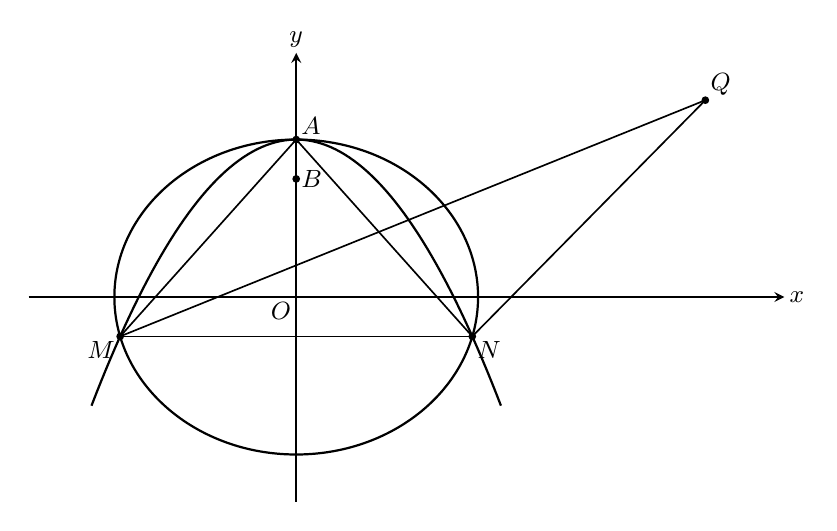
\begin{tikzpicture}[semithick, scale=1.0, every node/.style={inner sep=1.6pt, font=\small}]
  \draw[-stealth] (-3.4,0) -- (6.2,0) node[right] {$x$};
  \draw[-stealth] (0,-2.6) -- (0,3.1) node[above] {$y$};
  % C1 椭圆：a=2.309, b=2
  \draw[thick] (0,0) ellipse (2.3094 and 2);
  % C2 抛物线 x^2 = 4-2y
  \draw[thick,domain=-2.6:2.6,samples=90] plot (\x,{2-(\x)*(\x)/2});
  \fill (0,2) circle (1.4pt) node[above right] {$A$};
  \fill (0,1.5) circle (1.4pt) node[right] {$B$};
  \fill (5.196,2.5) circle (1.4pt) node[above right] {$Q$};
  \fill (-2.236,-0.5) circle (1.4pt) node[below left] {$M$};
  \fill (2.236,-0.5) circle (1.4pt) node[below right] {$N$};
  \draw (-2.236,-0.5) -- (2.236,-0.5);
  \draw (0,2) -- (-2.236,-0.5);
  \draw (0,2) -- (2.236,-0.5);
  \draw (5.196,2.5) -- (-2.236,-0.5);
  \draw (5.196,2.5) -- (2.236,-0.5);
  \node[below left] at (0,0) {$O$};
\end{tikzpicture}
